Notes for video 11.mp4
\subsection*{Butterworth Filter}

Choose $C(\omega)$ for maximum flatness at $\infty$.

We want the taylor expansion about infinity to be maximum flat. 

Work with $P(1/\omega)$ and go for maximum flatness at "new DC". \\
You want a maximally flat approximation to zero. 
\begin{align*}
C(\omega) &= 1 \\
C(\omega) &= \frac{1}{1 + C_{2N}\omega^{2N}}
\end{align*}

\paulhint{See frame 15a taken at 3:24}\\
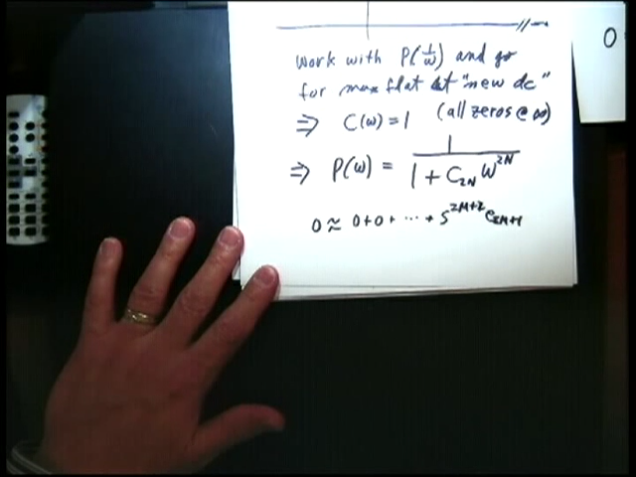
\includegraphics[scale=0.5]{frames/15a}


It's already a taylor series approximation starting at $2M + 2$.

Cutoff frequency gets changed by changing the C coefficient. \\

The more zeroes you have at inifity, the steeper the rolloff.  \\

\subsection*{Good for phase response}


\paulhint{See frame 15b taken at top chart.}\\
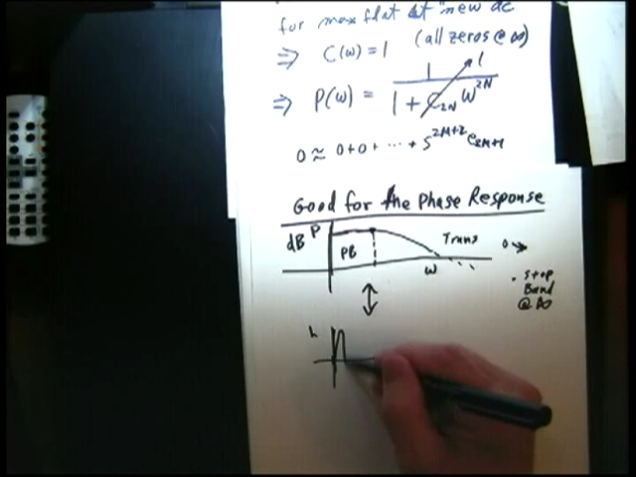
\includegraphics[scale=0.5]{frames/15b}

Maximally flat pass band, and a maximally slow transition band. There
isn't really a stop band, it's all transition band. Stop band is at inf, the
only place you make it to zero. Maximally gentle lowpass filter.  \\

The impulse response is going to be short:

\paulhint{See frame 15c. Short imp} \\
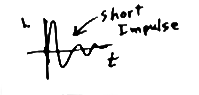
\includegraphics[scale=0.5]{frames/15c}

Short means, there isn't much phase distortion. \\

Suppose you put an impulse into the LPF filter: 

\paulhint{See frame 15d. Little diagram with LPF box} \\
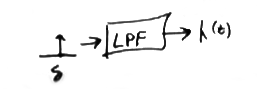
\includegraphics[scale=0.5]{frames/15d}

Intuitively, the filter will take the broadband click and output a narrow
band click. It should not ring. If you hear a ring, it is phase distortion. 

The ideal lowpass filter has a "corner", and the sync function rings like
crazy at the cutoff. Think of that as delaying those components. 
Group delay has a huge spike at cutoff frequency and polezero diagrm.

%\paulhint{See frame 15e. Little diagram with sync box, pole zero 
%diagrams, and group delay} \\
%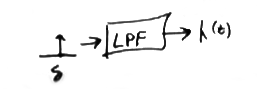
\includegraphics[scale=0.5]{frames/15d}

In the class of filters you often use, butterworth is the most friendly and
gentle to use. It's a nice smooth warm thing. Good thing to try first. 

$P(\omega) = \frac{1}{1 + \omega^{2N}}$ \\
$H(s)H(-s) = P(\omega) = P(\omega) \vert_{\omega = \frac{s}{j}}
= \frac{1}{1 + (\frac{s}{j})^{2N}}
$ \\

You might recognize this as roots of unity. A bunch of poles at the roots
of unity. Unit circle in the S-plane, which is where the poles of the butterworth
filter lie. 
\paulhint{See frame 15e. chart} \\
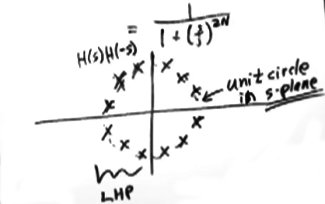
\includegraphics[scale=0.5]{frames/15e}

Poles are at 2nth roots of unity for odd N, else rot($pi/wN$).

Take the spectral factorization:  \\
LHP: \\
$H(s) = \frac{1}{(s - p_1) \cdots (s- p_n)}$
\paulhint{See frame 15g. for H(s) eqn} \\
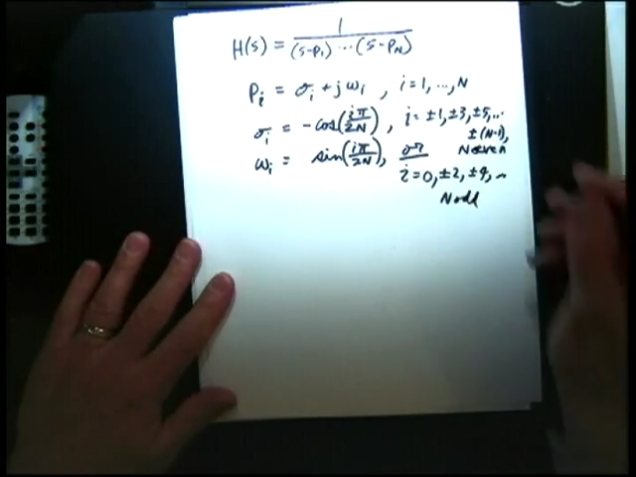
\includegraphics[scale=0.5]{frames/15g}

Intuitively, $N =1$, real pole, and minus s is mirrored at roots of unity.\\

\paulhint{graph is being written for N = 1 15h}\\
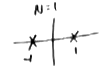
\includegraphics[scale=0.9]{frames/15h}

When $N = 2$, you get into trouble when you get roots of unity would be like
the DFT case, so you rotate the poles:\\

  
\paulhint{graph is being written for N = 2 15i}\\
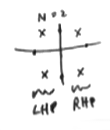
\includegraphics[scale=0.9]{frames/15i}


\subsection*{Series Biquad Realization}

The poles are in closed form, so we can easily take a series biquad realization.

\paulhint{Stonehenge like graphics. screenshot taken at 23:38 15j}

Elliptic function filter design are hard. Will NOT be covered in class. 


\paulhint{graph is being written for N = 2 15j}\\
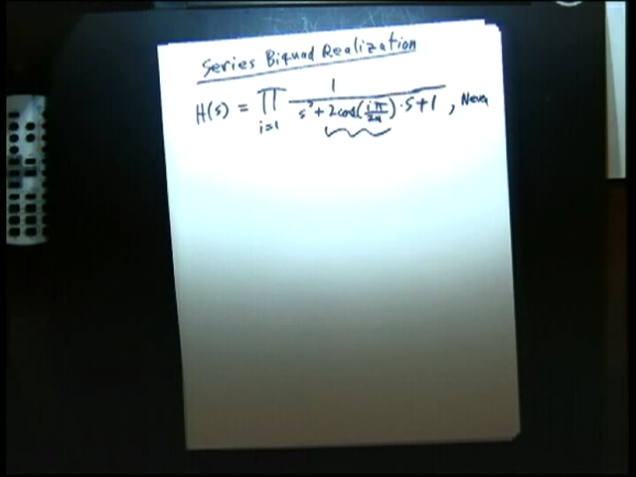
\includegraphics[scale=0.9]{frames/15j}\\
